\documentclass[11pt]{article}
\usepackage[margin=1in]{geometry}
\usepackage{booktabs}
\usepackage{graphicx}
\usepackage{longtable}
\usepackage[hidelinks]{hyperref}
\usepackage{url}
\usepackage{microtype}

\title{Merge by Kind, Commit by Hand:\\The BlobFS File Format}
\author{Kenneth Santala}
\date{}

\begin{document}
\maketitle

\begin{abstract}
BlobFS is a file system where files are living blobs that attract, merge, and split.
The contribution is narrow and specific.
Merging as a recorded storage operation is not new (Git, Irmin, Ficus and Coda all do forms of it); to our knowledge, no prior system combines four things:
(1) kind-typed fusion of distinct objects into a new stored container,
(2) refused merges recorded as events,
(3) propose-only operation with a human commit enforced at the storage layer, and
(4) a self-describing per-object archive with content-addressed payloads.
The \texttt{.orb} format stores real payloads deduplicated by SHA-256 hash.
\texttt{orb.py}, a stdlib Python reference written to the shipped format, and the browser loader agree on all 22 blob and 20 object hashes of \texttt{demo.orb}, and files written by each open in the other.
We do not claim BlobFS beats folders: the personal-file literature strongly favors browsing, and BlobFS builds nesting rather than removing it.
We present the format, the merge rules, and the test results; a user study comparing BlobFS in 3D, BlobFS in 2D, and ordinary folders is planned future work and has not been run.
\end{abstract}

\section{Introduction}

Folders are a filing-cabinet metaphor from the eighties.
They work because the same person both files and retrieves, and browsing beats searching by nearly three to one in dual-task experiments~\cite{bergman2013}.
But the metaphor has a cost: organization is a chore you do by hand, and the structure you build is brittle.

BlobFS inverts the relationship.
Files are blobs with mass, kind, and tags.
Similar files attract each other; when they touch, the format proposes a merge; a person confirms or refuses; and the result is a new stored object with history.
The disk organizes itself around what you actually do, and every fusion is reversible.

The contribution is not 3D, not physics, not self-organization, and not merge as a storage operation on its own.
All of those have ancestors~\cite{fsnwiki,agarawala2006,mander1992,farinier2015,reiher1994,kumar1995}.
The claim is narrow: to our knowledge, no prior system combines
(1) kind-typed fusion of distinct objects into a new stored container,
(2) refused merges recorded as events,
(3) propose-only operation with a human commit at the storage layer, and
(4) a self-describing per-object archive with content-addressed payloads.

\begin{figure}[t]
  \centering
  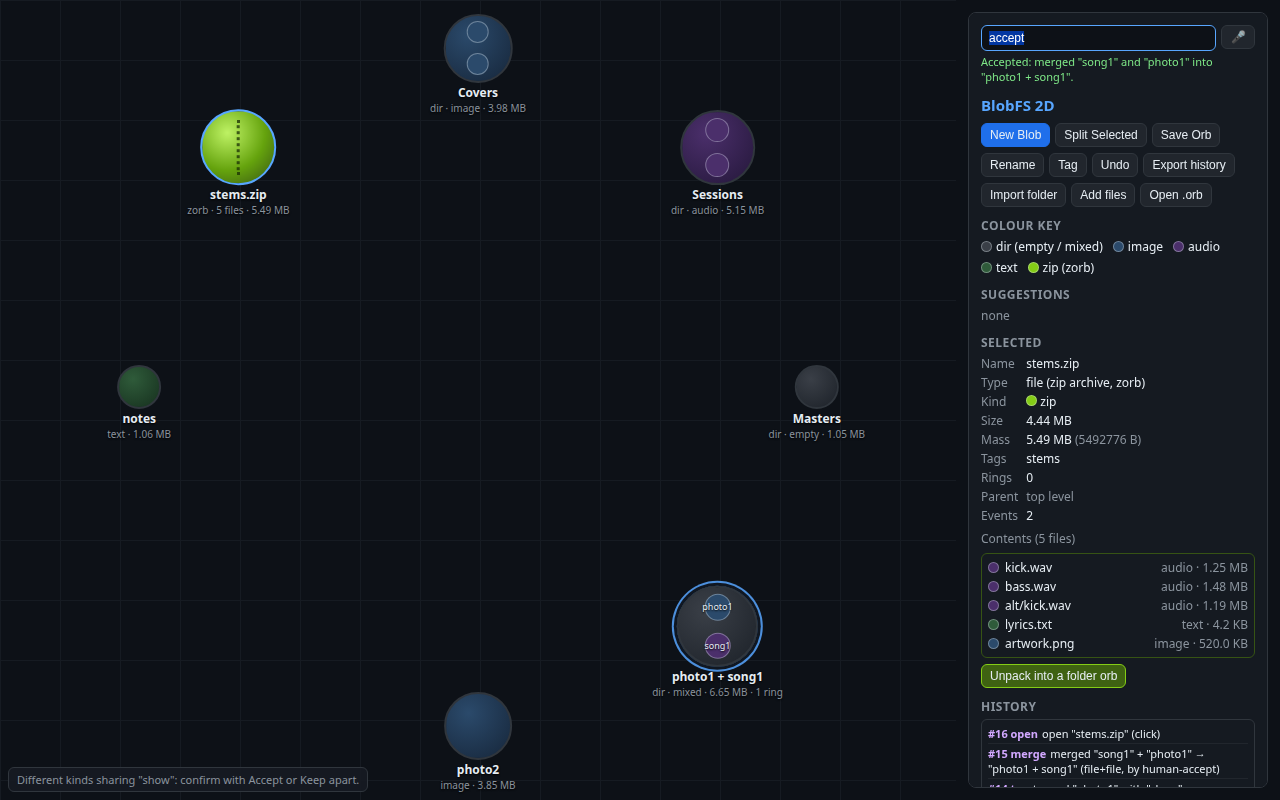
\includegraphics[width=0.92\linewidth]{figures/blobfs-2d.png}
  \caption{The 2D prototype (\texttt{blobfs-2d.html}) with the sample disk on a dark canvas. The lime orb \texttt{stems.zip} is open in the inspector, which lists five zip entries (two audio, one text, one image). Same-kind orbs share a colour. This is a screenshot of the page, not a measured result.}
  \label{fig:prototype}
\end{figure}

\section{Related Work}

Merging as a recorded, reversible storage operation is not new on its own.
Git merge commits, Irmin~\cite{farinier2015}, Ficus~\cite{reiher1994} and Coda~\cite{kumar1995} all do forms of it.
Earlier grouping systems kept the grouping in the interface or in queries, and version-control stores record merges of versions of the same content.

\subsection{Piles and physics desktops}

Piles~\cite{mander1992} and BumpTop~\cite{agarawala2006} grouped files by putting them together rather than naming a folder.
BumpTop gave objects mass and friction and merged piles with a lasso gesture; the granted patent covers that interface, not a storage format that records merge or refuse events~\cite{agarawala2013patent}.
In both systems the grouping lives in the interface.
In BlobFS the merge is an operation of the storage format, with recorded history and a human commit gate.

\subsection{3D and spatial file browsing}

3D file views date to the early 1990s (fsn on SGI IRIX~\cite{fsnwiki}).
Data Mountain~\cite{robertson1998} showed spatial placement can help retrieval.
Cockburn and McKenzie~\cite{cockburn2002} found 3D slowed it (3.7\,s in 2D vs.\ 4.8\,s in 3D).
FOLDER3D~\cite{luz2010} kept the folder tree on purpose.
The safe framing: BlobFS's contribution is the merge operation; 3D is one possible interface, and a 2D version of the same format is the fair control.
Figure~\ref{fig:prototype} is that 2D page.

\subsection{Beyond the hierarchy}

Semantic File Systems~\cite{gifford1991}, Lifestreams~\cite{fertig1996}, Placeless Documents~\cite{dourish2000}, and KondoCloud~\cite{brackenbury2021} group files by query, time, or property and leave the files untouched.
KondoCloud's 59 participants accepted 25.5\% of 1,856 suggestions.
That figure is taken from the paper as cited; it is treated here as a design input: suggestions are mostly refused, so physics may propose and cannot commit.
TagFS~\cite{bloehdorn2006} makes directories dynamic views over tags.
It is a view layer, not a storage operation.

\subsection{Storage side}

Venti~\cite{quinlan2002} identified blocks by content hash.
Fossil~\cite{quinlanfossil} layered a snapshotting Plan~9 file server over it.
Data Domain~\cite{zhu2008} made hash-based deduplication fast at backup scale.
The \texttt{.orb} store borrows the idea, not the scale: it dedups whole payloads per archive.
Elephant~\cite{santry1999} and CVFS~\cite{soules2003} kept old versions of one file, not fusions of different ones.
PASS~\cite{muniswamy2006} records provenance automatically.
The \texttt{.orb} log is closer to a user-decision log than to lineage capture.

\subsection{Merge as a storage operation}

Git merge commits and \texttt{git revert} already make merge a recorded, reversible storage operation.
Irmin generalizes it to typed data structures with three-way merge.
Ficus and Coda select type-specific resolvers to merge conflicting replicas of the same file.
Harmony~\cite{foster2007} uses schemas to synchronize replicas of structured data.
FileWeaver~\cite{gori2020} merges format variants of one file into a polymorphic ``morph'' and tracks dependencies.
All of these merge versions or variants of the same object.
Perkeep~\cite{perkeep} has content-addressed blobs and no merge operation.
overlayfs~\cite{overlayfs} and Unionfs~\cite{wright2006} merge directories as a namespace view over unchanged branches.
Ori~\cite{mashtizadeh2013} grafts a subtree between file systems while preserving history.
YoloFS~\cite{zhong2026} stages file-system mutations made by AI agents until a person commits them.
It is the closest prior on the human-commit axis, and it does not fuse distinct objects, log refused merges, or gate by kind.
\emph{Merge What You Can, Fork What You Can't}~\cite{schiefer2022} is an application-layer argument for keeping a failed merge visible, not a file-system prior.

Recent neighbours do not make fusion the primitive.
SYSSPEC~\cite{liu2026} generates file-system code from specifications.
LSFS~\cite{shi2025} groups by query.
LlamaFS~\cite{llamafs2024} renames and categorizes with accept-or-reject suggestions.
None fuses distinct objects into a stored container.

The personal-file literature strongly favours browsing folders~\cite{bergman2016,bergman2013}.
BlobFS fits that finding if it is framed correctly: every merge creates nesting, and the contents can be browsed level by level.
Mixed-initiative principles~\cite{horvitz1999,amershi2019} are the reason a suggestion waits for a person.

\section{The .orb Format}

An \texttt{.orb} file is a zip archive.
Inside: a magic header, then records.
Each blob is a record with an id, kind (file or directory), name, mass, children, and a content hash.
Child links are separate records pointing parent to child.
Merge events are their own record type.
Positions live in a separate record type, deliberately decoupled from identity.

Payloads are stored once under their SHA-256 hash in an \texttt{objects/} directory.
Identical bytes are stored once: three files with one duplicate became two payloads.
A flipped bit is caught when the orb is opened.
Name collisions get a disambiguator: \texttt{notes.txt} and \texttt{notes.txt} become \texttt{notes.txt} and \texttt{notes (2).txt}.
A folder merged into another goes in as a sub-orb, not flattened.
Undo is a new event that leaves the merge visible in the history.

The format is implemented twice: \texttt{blobfs-2d.html}, which reads and writes the zip with its own inline reader and writer, and \texttt{orb.py}, a stdlib-only Python reference (\texttt{zipfile}, \texttt{hashlib}, \texttt{json}) written afterwards to the format the page ships.
The cross-language test opens the committed \texttt{demo.orb} in \texttt{orb.py} and in the page's loader, headless in Chromium and Firefox.
Both sides agree on all 22 blob hashes, all 20 object hashes, the 13 links and the 101-record count.
A file written by \texttt{orb.py} opens in the page, and a file saved by the page opens and verifies in \texttt{orb.py}, with a random 70,001-byte payload compared byte for byte and a 50,000-byte file dropped onto the page compared by SHA-256.

\section{Merge Rules}

Three merge rules, so a drag never destroys data:
\begin{itemize}
  \item Directory $\cup$ directory becomes one directory. Children are kept.
  \item File $\cup$ file becomes a new directory holding both files, not a byte-level paste.
  \item File $\cup$ directory adopts the file as a child and adds its mass.
\end{itemize}
Mass is content size plus a constant $C = 1{,}048{,}576$ bytes, so an empty folder still has a body.
Radius follows the cube root of mass.

The kind gate: same-kind attraction is the default.
Cross-kind fusion requires explicit shared tags plus a human confirm.
Physics cannot commit a suggestion.
Refusing it leaves both blobs whole, and the refusal stays in the history.

\section{Evaluation}

The test suite covers the rules directly.
Each line below is checked by \texttt{tests/test\_orb.py} (20 tests), \texttt{tests/test\_crosslang.py} (12 tests), \texttt{tests/browser\_suite.js} (106 checks per browser), or more than one of those.
\begin{itemize}
  \item Split math is exact. A file of 2,700,000 bytes and a file of 800,000 bytes merged, then split: the parent lost exactly the child's mass, $800{,}000 + C = 1{,}848{,}576$ bytes, and parent mass plus child mass equaled the merged mass. Half of the two payload sizes is 1,750,000 bytes. That half is neither child's size, and it is not the mass that moved.
  \item The gate works both ways. With no shared tag, orbs held in contact are not proposed and are not merged. With a shared tag, a suggestion forms and waits. Physics can propose and cannot commit. A same-kind drop commits as \texttt{human-drop}. A refusal is recorded.
  \item Dedup: three files with one duplicate stored two payloads.
  \item Round-trip: every file's bytes identical after open-and-extract; same ids, same tree.
  \item Integrity: a flipped payload whose zip CRC was recomputed is refused as a hash mismatch, and a CRC-header flip is refused as a CRC mismatch. The page opens a DEFLATE archive written by Python. The page's inline SHA-256 matches the known digest of ``abc''.
  \item Collisions, nesting, and history behave as the format section says: a name clash keeps both payloads, a nested folder stays a sub-orb, and unmerge leaves the merge event in the log.
\end{itemize}

On 2026-10-19 both browsers passed 106/106 with zero console messages, page errors, or network requests (Chromium 11.245\,s, Firefox 16.026\,s, suite-reported, one run each).
That run was on a shared Linux VM with 4 vCPUs reported as ``Intel(R) Xeon(R) Processor'', 15\,GiB RAM, Ubuntu 24.04.5, Node v22.23.3, Playwright 1.56.1, Chromium 141.0.7390.37, and Firefox 142.0.1.
The same day, \texttt{python3 -m unittest} of the two Python modules passed 32/32 in 15.849\,s (one run) and again tallied 140 blob hashes, 128 object hashes, 84 links, and 8 page runs.

The 4\,GiB refusal is checked two ways.
One check still passes a File-like stub of size $2^{32}$ to \texttt{BlobFS.addFiles}, which reads only \texttt{.size}.
The other creates a sparse file with \texttt{truncate -s 4294967296} and hands that path to the page's file input.
The \texttt{stat} block count was 0 before and after, and the file was not added.
A separate one-run probe the same day, not one of the 106 checks, timed that input at 28\,ms in Chromium and 82\,ms in Firefox; \texttt{du -B1} reported 0 bytes allocated.
Spoken commands are not audio and not a microphone.
Playwright installs a fake \texttt{SpeechRecognition} before the page loads.
A scripted \texttt{open notes} is logged as \texttt{open "notes" (voice)}.
A scripted \texttt{new folder Spoken} creates that folder.
A scripted \texttt{not-allowed} error reports that microphone permission was denied and adds nothing.

Earlier suite runs are historical and were not repeated as part of the 2026-10-19 pass.
The original 73-check script (2026-10-03) was not kept, so its runtime was never recorded.
A 60-check rebuild on 2026-10-11 passed 60/60 in three runs per browser.
A 101-check run on 2026-10-16 passed 101/101 once per browser (Chromium 10.94\,s, Firefox 16.57\,s) on a 4\,vCPU VM.
The day-by-day table is in \texttt{paper/blobfs-paper.md}.
Those rows are the record of those runs.
They are not the current suite.

\subsection{Open time}

The 2026-10-11 open-time series used a shared Linux VM with 8 vCPUs, 15\,GiB RAM, and Python 3.13.5.
A small script's warm \texttt{orb.load} medians of five runs were 3.8\,ms (100 files), 40.7\,ms (1,000), and 193.3\,ms (4,000).
\texttt{demo.orb} (101 records) opened in 6.5\,ms (single run).
Browser and cold-cache numbers from that machine are in \texttt{bench/results-2026-10-11.txt} and \texttt{bench/results-cold-2026-10-11.txt}.
They are not repeated here as if they were the 2026-10-19 run.

The same scripts were run again on 2026-10-19 (\texttt{bench/run\_all.sh} and \texttt{bench/run\_cold.sh}).
This machine has 4 vCPUs reported as ``Intel(R) Xeon(R) Processor'', 15\,GiB RAM, Ubuntu 24.04.5, Python 3.12.3, Node v22.23.3, Playwright 1.56.1, Chromium 141.0.7390.37, and Firefox 142.0.1.
Disk byte sizes were 228{,}060, 2{,}305{,}070, 9{,}289{,}070, and 104{,}858{,}694.
Medians of 5 runs (min--max), in milliseconds.
Warm page cache:

\begin{center}
\small
\begin{tabular}{lrrrr}
\toprule
Disk & size & orb.py & Chromium & Firefox \\
\midrule
100 files & 0.23 MB & 4.1 (3.8--6.1) & 37 (36--41) & 22 (20--23) \\
1,000 files & 2.3 MB & 40.2 (38.5--46.0) & 206 (202--313) & 192 (189--220) \\
4,000 files & 9.3 MB & 166.6 (163.6--188.2) & 1{,}763 (1{,}726--2{,}923) & 1{,}732 (1{,}701--1{,}779) \\
1 file, 100 MiB & 104.9 MB & 151.1 (148.1--188.7) & 658 (649--665) & 1{,}337 (1{,}326--1{,}349) \\
\bottomrule
\end{tabular}
\end{center}

Cold cache, same day, after the warm series.
Before every timed run the script dropped the guest page cache, then \texttt{mincore} reported 0 resident bytes of the \texttt{.orb} on all 60 runs.
Cold means cold in this guest's page cache.
The host may still cache the virtio disk.

\begin{center}
\small
\begin{tabular}{lrrrr}
\toprule
Disk & size & orb.py & Chromium & Firefox \\
\midrule
100 files & 0.23 MB & 5.3 (4.8--6.0) & 41 (39--50) & 25 (22--49) \\
1,000 files & 2.3 MB & 43.4 (41.5--48.5) & 370 (345--425) & 209 (206--218) \\
4,000 files & 9.3 MB & 192.0 (183.5--208.6) & 1{,}954 (1{,}848--2{,}026) & 1{,}928 (1{,}894--2{,}043) \\
1 file, 100 MiB & 104.9 MB & 204.4 (197.8--209.4) & 756 (750--783) & 1{,}452 (1{,}446--1{,}524) \\
\bottomrule
\end{tabular}
\end{center}

These 2026-10-19 guest numbers are not a comparison against the 8-vCPU 2026-10-11 machine.

The same scripts also ran once on a GitHub-hosted runner on 2026-10-19.
Workflow run 39296171414 (\texttt{benchmarks} / job \texttt{open-time}) started at 2026-10-19T17:40:46Z and finished successfully.
The job recorded its environment at 2026-10-19T17:41:25Z: 4 vCPUs, model name INTEL(R) XEON(R) PLATINUM 8573C, 15\,GiB RAM, Ubuntu 24.04.5 LTS, kernel 6.17.0-1022-azure, Python 3.12.15, Node v20.20.2, Playwright 1.56.1.
That Playwright release installs Chromium 141.0.7390.37 and Firefox 142.0.1, and the job ran \texttt{npx playwright install --with-deps chromium firefox}.
Raw logs are \texttt{bench/results-gha-2026-10-19.txt} and \texttt{bench/results-cold-gha-2026-10-19.txt}.
Disk byte sizes matched the local disks.
Medians of 5 runs (min--max), in milliseconds.
Warm page cache:

\begin{center}
\small
\begin{tabular}{lrrrr}
\toprule
Disk & size & orb.py & Chromium & Firefox \\
\midrule
100 files & 0.23 MB & 6.0 (5.7--7.5) & 56 (55--66) & 29 (28--41) \\
1,000 files & 2.3 MB & 59.4 (57.6--64.6) & 494 (437--500) & 268 (260--273) \\
4,000 files & 9.3 MB & 254.7 (251.5--259.4) & 2{,}403 (2{,}352--5{,}618) & 2{,}367 (2{,}351--2{,}400) \\
1 file, 100 MiB & 104.9 MB & 155.3 (154.1--156.6) & 754 (749--758) & 1{,}572 (1{,}546--1{,}592) \\
\bottomrule
\end{tabular}
\end{center}

Chromium's five warm runs on the 4,000-file disk were 5{,}618, 4{,}181, 2{,}403, 2{,}352, and 2{,}397\,ms.
The median is 2{,}403\,ms.
The first two runs are the high end of that range.

Cold cache, same job, after the warm series.
Before every timed run the script dropped the runner's page cache, then \texttt{mincore} reported 0 resident bytes of the \texttt{.orb} on all 60 runs.

\begin{center}
\small
\begin{tabular}{lrrrr}
\toprule
Disk & size & orb.py & Chromium & Firefox \\
\midrule
100 files & 0.23 MB & 7.7 (7.5--9.0) & 70 (60--90) & 44 (33--46) \\
1,000 files & 2.3 MB & 66.1 (63.2--71.1) & 458 (448--487) & 292 (290--296) \\
4,000 files & 9.3 MB & 267.8 (265.8--281.7) & 2{,}451 (2{,}416--2{,}505) & 2{,}357 (2{,}310--2{,}422) \\
1 file, 100 MiB & 104.9 MB & 522.8 (521.7--526.8) & 1{,}081 (1{,}072--1{,}109) & 1{,}879 (1{,}877--1{,}892) \\
\bottomrule
\end{tabular}
\end{center}

The 2026-10-11 machine, the 2026-10-19 guest, and this GitHub-hosted runner are three different environments.
The tables are not a comparison between them.

\section{Planned User Study}

No user study has been run.
This section describes a planned study, and no results are reported or implied.
A small study with 12 to 16 people would use three interfaces in balanced order: BlobFS in 3D, BlobFS in a flat 2D view of the same format, and an ordinary folder window.
Each participant would organize about 60 files, and a day later find 15 files from short descriptions.
Measures would include search time and failures, merges, splits, undos, and the share of suggested merges accepted.
None of this has been carried out.
The study would need ethics approval.

\section{Limitations}

No user study yet.
The mass constant $C$ is a chosen value, not derived.
The repulsion coefficient is tuned, not derived.
Performance numbers are the small open-time benchmarks above, on two different shared VMs and one GitHub-hosted runner, and the browser-suite timings named with their dates.
The original 73-check script was not recovered.
The zip profile has not been formally specified.
There is no ZIP64.
A sparse file of exactly 4\,GiB was refused through the file input; a save that actually exceeds 4\,GiB in total was not built.
Sample-disk files are placeholders.
The related-work search used openly accessible records; IEEE Xplore full texts were not reviewed.
Eye tracking is not implemented.
Spoken commands were exercised with a fake Web Speech API, not a microphone.
3D delivery is future work.
The 2D prototype is a browser page.

\section{Conclusion}

BlobFS combines kind-typed fusion of distinct objects into a new stored container, refusals recorded as events, a human as the one who commits, and a self-describing archive with content-addressed payloads.
The format is real: two implementations agree, and the tests that were run passed.
What remains is the user study.
Nothing you merge should ever be gone for good.

\bibliographystyle{plain}
\bibliography{blobfs}

\end{document}
